\subsection{Share of Detected Cases}
\label{subsec:data_share_known_cases}

 \comment[id=K]{Stoye called this the ascertainment rate if I remember right. Maybe we should replace this everywhere}

One important feature of our model is that we distinguish between undetected and detected
cases and that we model which cases are detected and which are not (see \ref{sub:testing}
for a detailed description for how we model both rapid and PCR tests). For our model it
is important to have an estimate for the share of cases that is detected in the absence
of rapid tests. For this we rely on the
\href{https://covid19.dunkelzifferradar.de/}{Dunkelzifferradar} which relies on estimates
of the case fatality rate to estimate the number of total cases given the number of
deaths which are suspected to be perfectly observable. For 2020, we follow the reported
share of detected cases quite closely only interpolating the phase of November 2020 where
the testing policy was changed to give more priority to vulnerable groups. This lead to
more tests being done among older age groups which are also at the highest risk of dying
from CoViD-19 and an overestimation of the share of detected cases.
% After Christmas 2020
Similarly, the start of vaccinations after Christmas 2020 that were predominantly given
to nursing homes in the beginning and other vulnerable groups in spring, led to a
decrease in the number of deadly cases, leading to an increasing upward bias in the share
of detected cases. This is why we stop using the Dunkelzifferradar after Christmas.
Instead, we assume that that the share of detected cases would have stayed the same in
the absence of rapid tests. Thus, we also achieve in our model an increase in the share
of detected cases but this is driven from inside our model through increased testing and
follow-ups on positive rapid tests (see Section~\ref{subsec:results_share_known_cases}).
% Christmas and Easter
Lastly, we include reductions in the share known cases due to the two major holidays in
our simulation period, Christmas and Easter. During both holidays where many laboratories
do not process tests and most physicians' offices are closed, less PCR tests were done
leading to short and large drops in the share of known cases.

\begin{figure}[ht]
  \centering
  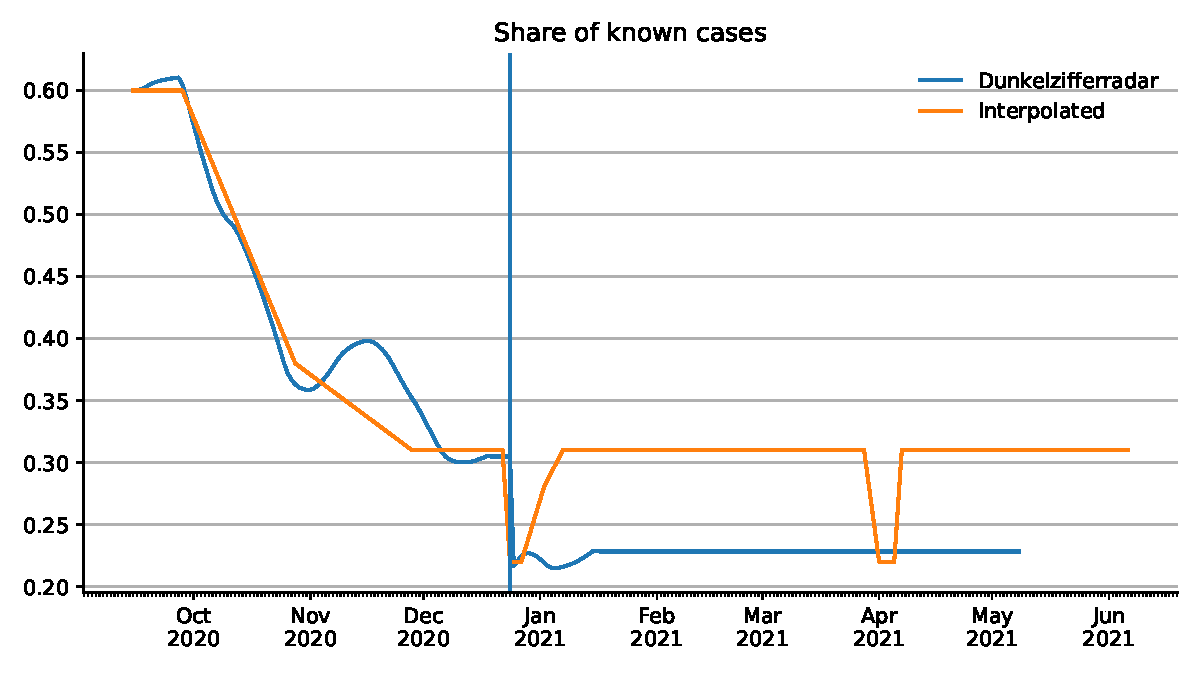
\includegraphics[width=\textwidth]{figures/results/figures/data/testing/assumed_overall_share_known_cases}
  \caption{Share of Detected Cases}
  \label{fig:share_known_cases_data}
  \floatfoot{\noindent \textit{Note:} The figure shows the share of cases that is
  reported as an official case via PCR confirmation. We use the overall share of known
  cases that was estimated through the case fatality ratio by the
  \href{https://covid19.dunkelzifferradar.de/}{Dunkelzifferradar} for all of 2020 and
  then assume it to be constant as vaccinations of the elderly strongly affect the case
  fatality rate which the project does not account for. Starting in 2021 in addition to
  the overall numbers of detected cases through symptoms and the share known cases, cases
  are also detected through confirmation of positive rapid tests which happens
  endogenously inside the model. For the public holidays of Christmas and Easter we lower
  the share of detected cases as fewer PCR tests are available during public holidays.}
\end{figure}

\FloatBarrier